\section{HuggingFace}
\label{research:HuggingFace}
As part of my preparation for my later practical project during the work experience I began researching different AI models to find the pros and cons of either. During this process I was mindful to learn not just about the specific models I would be using for my work experience project, but also about the differences between all sorts of Models and datasets 

I spent this time exploring sources such as Hugging Face \autocite{ModelsHuggingFace2025}(a community driven site dedicated to tracking the release and performance of various AI models, the existence of which fuels the growth and development of AI)  and reaching out to some contacts I have previously made (through prior work experiences and networking events). These sources helped me develop my understanding of the technologies responsible for so many recent innovations and proved to be hugely useful in aiding my learnings from my later research tasks. The Hugging Face source below for example ranks LLMs (Large Language Models) on a variety of criteria and is a useful resource for developers looking to maximise the abilities of their implementations with the processing resources they have available

\begin{figure}[H]
    \centering
    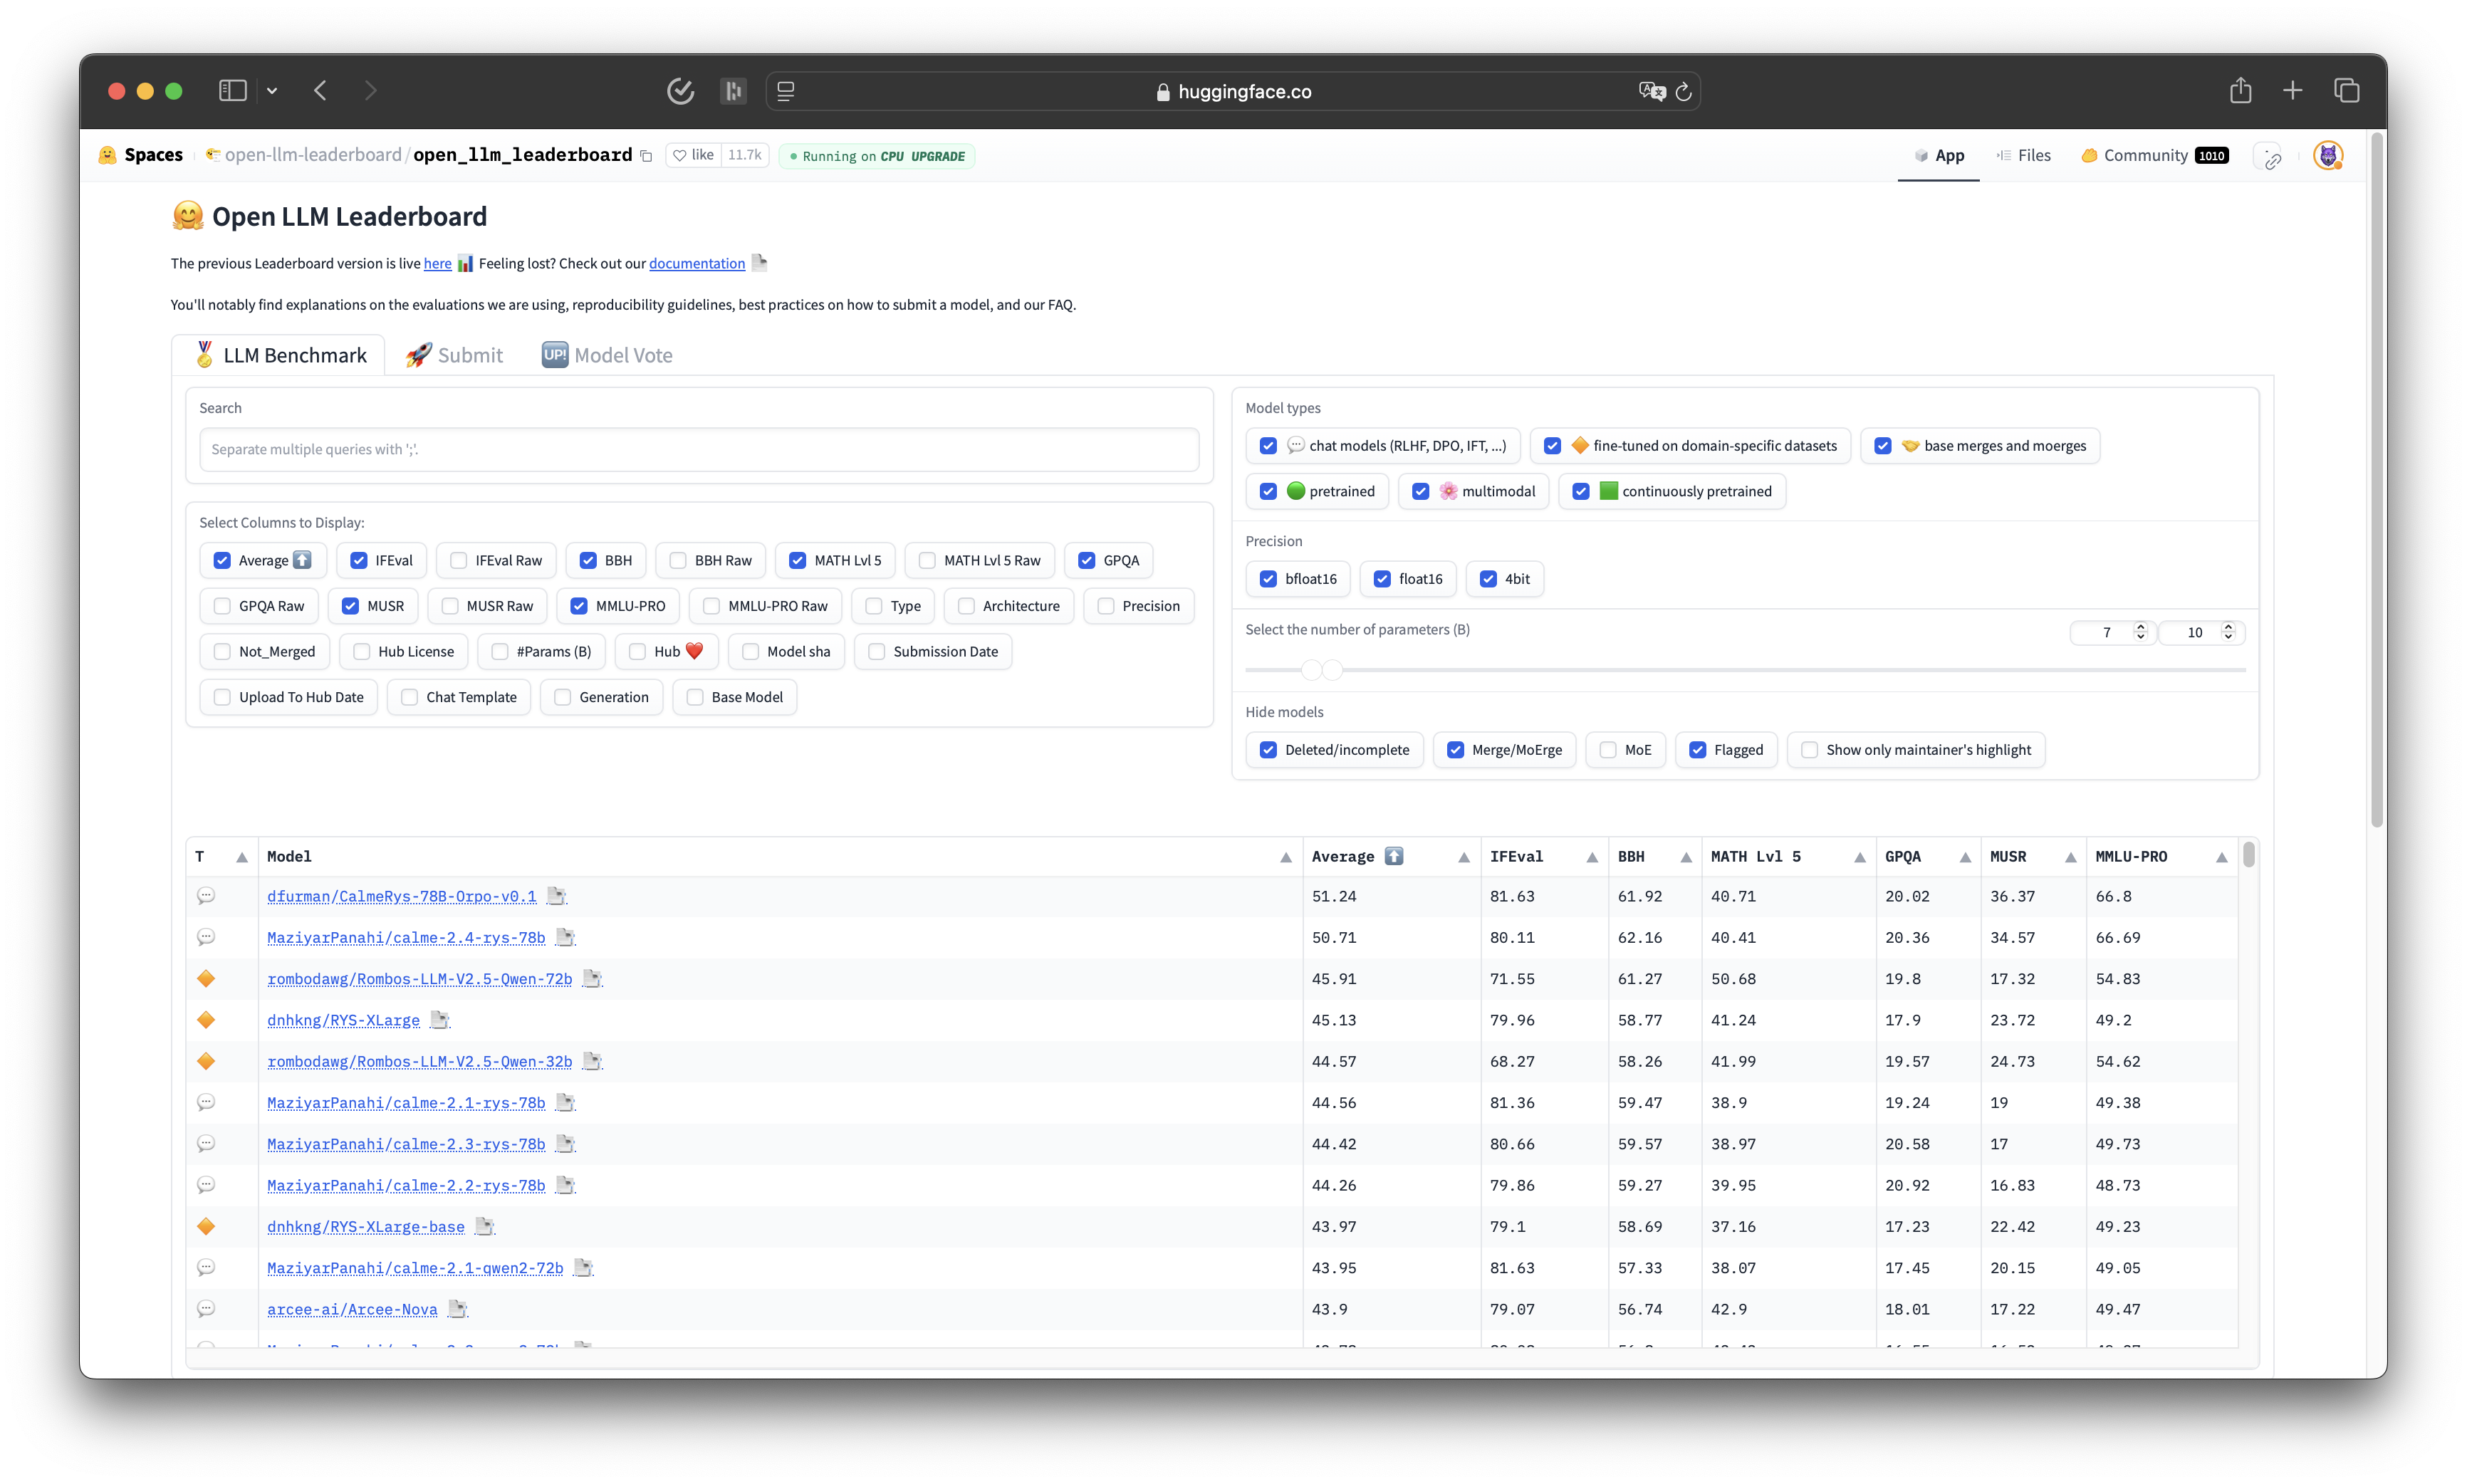
\includegraphics[width=0.8\textwidth]{Research/5_HuggingFace/media/HuggingFace.png}
    \caption{Overview of popular models listed on Hugging Face.}
    \label{fig:huggingface-models}
\end{figure}